\chapter{Discs}
\label{sec:Discs}
\section{Discs Potentials}

\begin{equation}
\Phi_M (R, z) = - \dfrac{GM}{\sqrt{R^2 + (a + \sqrt(z^2 + b^2))^2}}
\end{equation}

\begin{equation}
\rho_M (R, Z) = \left( \dfrac{b^2 M}{4 \pi} \right) \dfrac{aR^2 + (a + 3\sqrt{z^2+b^2})(a + \sqrt{z^2+b^2})^2}{[R^2 + (a^2 + \sqrt{z^2+b^2})^2]^{5/2}(z^2+b^2)^{3/2} }
\end{equation}


\begin{figure}[H]\label{fig:MN_density}
\centering
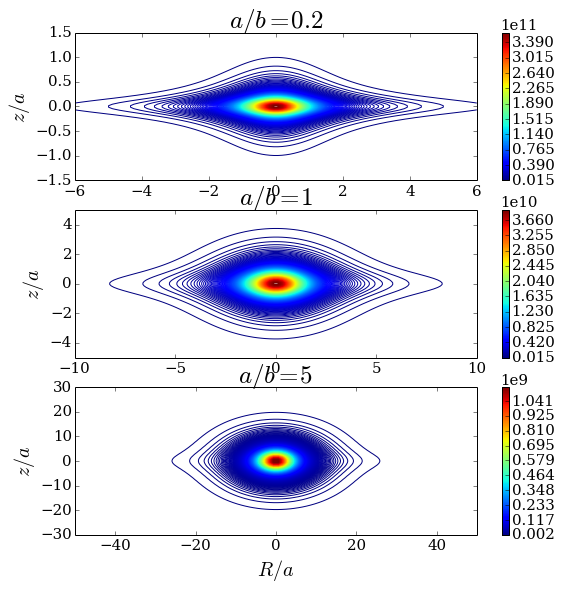
\includegraphics[scale=0.7]{../figures/MN_density_contours.png}
\end{figure}

\section{Logarithmic Profile}\label{sec:log}

Disc profile

\begin{equation}
\Phi_L(R, z) = \dfrac{1}{2} v_0^2 ln \left( R_c^2 + R^2 + \dfrac{z^2}{q_{\phi}^2}  \right) + constant
\end{equation}

The circular velocity at $z=0$ is $v_c^22(R, z=0) = r \dfrac{d \Phi}{dR}$:

\begin{equation}
v_c(R, z=0) = r \dfrac{d \Phi_L}{dr} = \dfrac{v_0 R}{\sqrt{r_c^2 + R^2}}
\end{equation}

\begin{figure}[H]
\centering
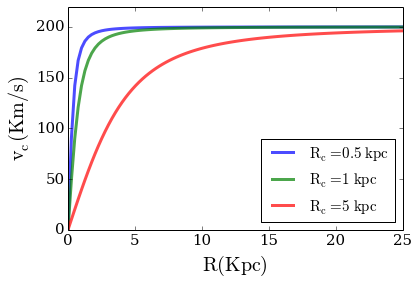
\includegraphics[scale=0.7]{../figures/Log_vc.png}
\end{figure}


To derive the density we make use of Poisson's equation in cylindrical coordinates:

\begin{equation}
\rho_L(R, z) = \dfrac{\nabla^2 \Phi_L}{4 \pi G } = \dfrac{1}{4 \pi G} \left( \dfrac{1}{r}\dfrac{d}{dR}R\dfrac{d}{dR}  + \dfrac{d^2}{dz^2}  \right) \Phi_L
\end{equation}

\begin{equation}
\rho_L(R, z) = \dfrac{v_0^2}{8 \pi G } \left( \dfrac{1}{R} \dfrac{4R ( R_c^2 + R^2 + \dfrac{z^2}{q_{\phi}^2} ) - 4R^3}{( R_c^2 + R^2 + \dfrac{z^2}{q_{\phi}^2} )^2} + \dfrac{\dfrac{2}{q_{\phi}^2} ( R_c^2 + R^2 + \dfrac{z^2}{q_{\phi}^2} ) - \dfrac{4z^2}{q_{\phi}^4}}{( R_c^2 + R^2 + \dfrac{z^2}{q_{\phi}^2} )^2}  \right)
\end{equation}

\begin{equation}
\rho_L(R, z) =  \dfrac{v_0^2}{4 \pi G q_{\phi}^2} \dfrac{(2q_{\phi}^2 + 1)R_c^2 + r^2 + (2 - q_{\Phi^2})z^2}{(R_c^2 + r^2 + z^2q_{\Phi}^{-2})^2}
\end{equation}


\begin{figure}[H]
\centering
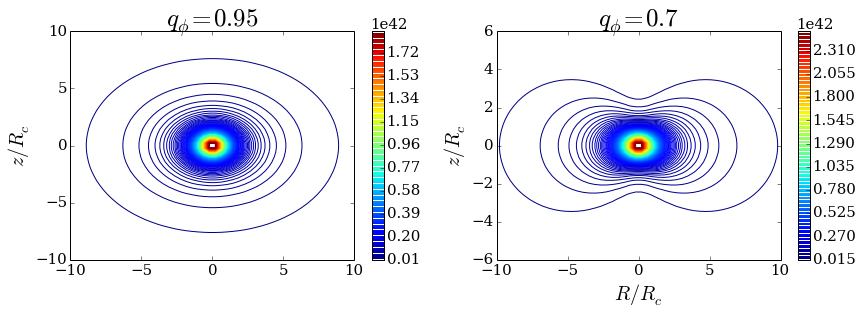
\includegraphics[scale=0.6]{../figures/MN_logarithmic_contours.png}
\end{figure}

